\documentclass[11pt, openright]{book}

    % Cover Variables
    \newcommand{\ctitle}{COMPTE-RENDU TP ELEN2}
    \newcommand{\cautor}{Author}
    \newcommand{\ctoptitle}{}

    % Header Variables
        \newcommand{\headRE}{\emph{\thepage}}
        \newcommand{\headLE}{\emph{\thesection. \rightmark}}
        \newcommand{\footRE}{}
        \newcommand{\footLE}{}

    % TOC Variables
        \newcommand{\toctitle}{Table of Content}
        \newcommand{\tocchapter}{Chapter}
        \newcommand{\toccount}{3}
  
    % Chapter Variables
        \newcommand{\chvar}{Chapter -}

\usepackage[a4paper, total={16cm, 22.125cm}]{geometry}

% Page Style
\usepackage[]{environ}
% Cover Page 
\usepackage{tikz}
\makeatletter
\def\parsecomma#1,#2\endparsecomma{\def\page@x{#1}\def\page@y{#2}}
\tikzdeclarecoordinatesystem{page}{
    \parsecomma#1\endparsecomma
    \pgfpointanchor{current page}{north east}
    % Save the upper right corner
    \pgf@xc=\pgf@x%
    \pgf@yc=\pgf@y%
    % save the lower left corner
    \pgfpointanchor{current page}{south west}
    \pgf@xb=\pgf@x%
    \pgf@yb=\pgf@y%
    % Transform to the correct placement
    \pgfmathparse{(\pgf@xc-\pgf@xb)/2.*\page@x+(\pgf@xc+\pgf@xb)/2.}
    \expandafter\pgf@x\expandafter=\pgfmathresult pt
    \pgfmathparse{(\pgf@yc-\pgf@yb)/2.*\page@y+(\pgf@yc+\pgf@yb)/2.}
    \expandafter\pgf@y\expandafter=\pgfmathresult pt
}
\makeatother


% Object formatting
\usepackage[12pt]{moresize}
\usepackage[]{anyfontsize}
\usepackage{titlesec}
\usepackage{import}
\usepackage{floatrow}
\usepackage{enumitem}
\usepackage{changepage}
\usepackage[normalem]{ulem}
\usepackage{array}
\newcommand{\ul}[1]{\underline{#1}}

\usepackage[]{chngcntr}
\usepackage{ifthen}
\ifthenelse{\figcountdepth > 1}
  {\counterwithin{figure}{section}\counterwithin{table}{section}}
  {}

\usepackage[format=plain, labelfont=it, textfont=it]{caption}
\makeatletter
\def\@makecaption#1#2{%
    \vskip\abovecaptionskip
    \sbox\@tempboxa{\textit{#1.} #2}

       
   

    \ifdim \wd\@tempboxa >\hsize
        #1. #2\par
    \else
        \global \@minipagefalse
        \hb@xt@\hsize{\hfil\box\@tempboxa\hfil}
    \fi
    \vskip\belowcaptionskip}
\makeatother

\DeclareCaptionFormat{underline}{\uline{#1#2#3}\par}

% Sections
\titleformat{\section}{\fontsize{16}{19.2}\bfseries}{\thesection.}{0.25em}{}
\titleformat{\subsection}{\fontsize{14}{16.8}\bfseries}{\tab\thesubsection.}{0.25em}{}
\titleformat{\subsubsection}{\fontsize{10}{12}}{\uline{\thesubsubsection)\enspace}}{0em}{\uline}





% Geometry

% Typewritting

\setlength{\parskip}{1em}
\setlength{\parindent}{0em}


\newenvironment{items}[3][0pt]
{\def\closesep{#3}
    \vspace{#2}
    \begin{itemize}
        \setlength{\itemsep}{#1}
        \setlength{\topsep}{0pt}
        \setlength{\partopsep}{0pt}}
        {\end{itemize}
    \vspace{\closesep}}

\newenvironment{enum}[3][0pt]
{\defclosesep{#3}
    \vspace{#2}
    \begin{enumerate}
        \setlength{\itemsep}{#1}
        \setlength{\topsep}{0pt}
        \setlength{\partopsep}{0pt}}
        {\end{enumerate}
    \vspace{\closesep}}

\newenvironment{eq}[2]
{\def\closesep{#2}
    \vspace{#1}
    \begin{align*}}
        {\end{align*}
    \vspace{\closesep}}

\newenvironment{lfeq}[2]
{\def\closesep{#2}
    \vspace{#1}
    \begin{flalign*}}
        {\end{flalign*}
    \vspace{\closesep}}
% List Formatting


\NewEnviron{dent}[1]{
    \vspace{-10pt}
    \begin{adjustwidth}{7mm}{}
        \uline{#1}\hspace{2mm}
        \BODY
    \end{adjustwidth}
    \vspace{-10pt}
}


\usepackage[framemethod=tikz]{mdframed}
\newcounter{count_theorem}[section]\setcounter{count_theorem}{0}
\newcommand{\thetheorem}{\arabic{count_theorem}}

\newcounter{count_exercise}[section]\setcounter{count_exercise}{0}
\newcommand{\theexercise}{\arabic{count_exercise}}


\newenvironment{theorem}[1][]{
    \refstepcounter{count_theorem}
    \mdfsetup{
        linecolor=red!30,
        innerbottommargin=10pt,
        linewidth=2pt,
        topline=false,
        bottomline=false,
        rightline=false,
        shadow=true,
        shadowsize=4.5pt,
        frametitlerule=false,
        apptotikzsetting={
                \tikzset{
                    mdfbackground/.append style={
                            left color=red!8,right color=red!3
                        }
                }
            }
    }
    \begin{mdframed}[]\relax
        \ifstrempty{#1}
        {\textbf{Theorem~\thetheorem.} }
        {\textbf{Theorem~\thetheorem.~#1} }
        }
        {\end{mdframed}\vspace{-10pt}
}

\newenvironment{note}{
    \mdfsetup{innertopmargin=5pt,
        linecolor=gray!30,
        linewidth=2pt,
        topline=false,
        bottomline=false,
        rightline=false,
        frametitleaboveskip=0pt,
        shadow=false,
        shadowsize=4pt,
        frametitlerule=false,
        apptotikzsetting={
                \tikzset{
                    mdfbackground/.append style={
                            left color=gray!8,right color=gray!3
                        }
                }
            }
    }
    \begin{mdframed}[]\relax
        \textbf{Note. }
        }
        {\end{mdframed}\vspace{-10pt}
}

\newenvironment{example}{
    \mdfsetup{innertopmargin=5pt,
        linecolor=green!30,
        linewidth=2pt,
        topline=false,
        bottomline=false,
        rightline=false,
        frametitleaboveskip=0pt,
        shadow=false,
        shadowsize=4pt,
        frametitlerule=false,
        apptotikzsetting={
                \tikzset{
                    mdfbackground/.append style={
                            left color=green!7,right color=green!2
                        },
                    mdfframetitlebackground/.append style={
                            left color=green!7,right color=green!2
                        }
                }
            }
    }
    \begin{mdframed}[]\relax
        \textbf{Example. }
        }
        {\end{mdframed}\vspace{-10pt}
}


\usetikzlibrary{calc,arrows}

\tikzset{
    excursus arrow/.style={%
            line width=2pt,
            draw=gray!40,
            rounded corners=2ex,
        },
    excursus head/.style={
            fill=white,
            font=\bfseries\sffamily,
            text=gray!80,
            anchor=base west,
        },
    excursus line/.style={%
            line width=2pt,
            draw=gray!40,
            rounded corners=2ex,
        }
}

\newenvironment{exercise}[1][]{%
    \refstepcounter{count_exercise}
    \mdfsetup{
        singleextra={
                \path let \p1=(P), \p2=(O) in (\x2,\y1) coordinate (Q);
                \path let \p1=(Q), \p2=(O) in (\x1,{(\y1-\y2)/2}) coordinate (M);
                \path [excursus line] ($(O)+(5em,0ex)$) -| (M) |- ($(Q)+(20em,0ex)$);
                \node [excursus head] at ($(Q)+(2.5em,-0.75pt)$) {\ifstrempty{#1}{Exercise \theexercise}{Exercise \theexercise:~#1}};},
        firstextra={
                \path let \p1=(P), \p2=(O) in (\x2,\y1) coordinate (Q);
                \path [excursus arrow,-to] (O) |- ($(Q)+(12em,0ex)$) .. controls +(0:16em) and +(185:6em) .. ++(23em,2ex);},
        middlelinewidth=2.5em,middlelinecolor=white,
        hidealllines=true,topline=true,
        innertopmargin=0.5ex,
        innerbottommargin=2.5ex,
        innerrightmargin=2pt,
        innerleftmargin=2ex,
        skipabove=0.87\baselineskip,
        skipbelow=0.62\baselineskip,
    }
    \begin{mdframed}[]\relax}
        {\end{mdframed}\vspace{-10pt}
}

% Functions and Data Plotting
\usepackage{subfig,wrapfig,adjustbox,multirow}


% Plotting Style
\usepackage{graphicx,pgfplots}
\usetikzlibrary{arrows}
\usetikzlibrary {patterns,patterns.meta}
\usepgfplotslibrary{fillbetween}
\pgfplotsset{compat=1.18}

\usepgfplotslibrary{units}
% Logarithmic Scale
\pgfplotsset{
    log x ticks with fixed point/.style={
            xticklabel={
                    \pgfkeys{/pgf/fpu=true}
                    \pgfmathparse{exp(\tick)}%
                    \pgfmathprintnumber[fixed relative, precision=3]{\pgfmathresult}
                    \pgfkeys{/pgf/fpu=false}
                }
        }
}


% Mathematics

% Formatting
\usepackage{amsmath}
\usepackage{esvect}
\usepackage{amsfonts}
\usepackage{tasks,environ}
\usepackage{xargs}
\usepackage{esint}
\usepackage[]{listings}


\usepackage[english]{babel}
\usepackage{amsthm}
%\newtheorem{theorem}{Theorem}
%\newtheorem{proof}{Proof}



%Custom Shortcuts
\newcommand{\eqi}{\Leftrightarrow}
\newcommand{\lr}[1]{\left( #1 \right)}
\newcommand{\limit}[1]{\displaystyle{\lim_{#1}}}
\newcommand{\tab}{\hspace*{7mm}}
\newcommand{\ds}[1]{\displaystyle{#1}}
\newcommand{\floor}[1]{\lfloor #1 \rfloor}
\newcommand{\R}{\mathbb{R}}
\newcommand{\N}{\mathbb{N}}
\newcommand{\Z}{\mathbb{Z}}
\newcommand{\C}{\mathbb{C}}
\newcommand{\K}{\mathbb{K}}
\newcommand{\F}{\mathcal{F}}
\newcommand{\M}{\mathcal{M}}
\renewcommand{\l}{\lambda}
\newcommand{\seg}[1]{\overline{\rm {#1}}}
\newcommand{\Int}{\int\limits}
\newcommand{\ex}{\tab \uline{Example :}\hspace{0.2cm} }
\newcommand{\vard}{\partial}
\newcommand{\Q}{\mathcal{Q}}
\newcommand{\Vect}{\operatorname{Vect}}
\newcommand{\rg}{\operatorname{rg}}
\renewcommand{\dim}{\operatorname{dim}}
\renewcommand{\Re}{\operatorname{Re}}
\renewcommand{\Im}{\operatorname{Im}}
\renewcommand{\P}{\mathcal{P}}
\newcommand{\blr}[1]{\left\{#1\right\}}
\newcommand{\linecenter}[1]{\par\vspace{2mm} \centerline{#1}\par\vspace{-2mm}}
\newcommand{\dd}{\textrm{d}}
\newcommand{\supp}{\operatorname{Supp}}
\renewcommand{\vec}{\overrightarrow}
\renewcommand{\epsilon}{\varepsilon}

% Matrix Configurations

\makeatletter
\renewcommand*\env@matrix[1][*\c@MaxMatrixCols c]{%
    \hskip -\arraycolsep
    \let\@ifnextchar\new@ifnextchar
    \array{#1}}
\makeatother


% Colors
\usepackage{xcolor}
\newcommand{\blu}{\color{blue}}
\newcommand{\Red}{\color{red}}
\newcommand{\blac}{\color{black}}

\newcommand{\red}[1]{\textcolor{red}{#1}}

\usepackage{xcolor,xspace}
\usepackage{breqn}


% Headings  
\usepackage[Glenn]{fncychap}
\ChNumVar{\fontsize{40}{42}}
\ChTitleVar{\Large\sc}
\ChNameVar{\Large\sc}
\setlength\headheight{14.5pt}
\renewcommand\FmN[1]{\chvar}



\usepackage{fancyhdr}
\usepackage{ragged2e}

% Header & Footers
\renewcommand{\chaptermark}[1]{\markboth{#1}{#1}}
\renewcommand{\sectionmark}[1]{
    \markright{ #1}
}
\pagestyle{fancy}
\fancyhf{}
\fancyhead[LE,RO]{\headLE}
\fancyhead[RE,LO]{\headRE}
\fancyfoot[LE,RO]{\footLE}
\fancyfoot[RE,LO]{\footRE}
\renewcommand{\headrulewidth}{0.5pt}
\fancyheadoffset{1cm}

\fancypagestyle{plain}{%
    \fancyhf{} % clear all header and footer fields
    \fancyfoot[LE, RO]{\footLE}
    \renewcommand{\headrulewidth}{0pt}
    \renewcommand{\footrulewidth}{0pt}}


\fancypagestyle{nohead}{%
    \fancyhf{} % clear all header 
    \fancyfoot[LE, RO]{\footLE}
    \fancyfoot[LO, RE]{\footRE}}

    \fancypagestyle{head}{%
    \fancyhf{} % clear all header 
    \fancyhead[LE,RO]{\headLE}
\fancyhead[RE,LO]{\headRE}
\renewcommand{\headrulewidth}{0.5pt}
\fancyheadoffset{1cm}
    }


\fancypagestyle{bib}{%
    \fancyhf{} % clear all header and footer fields
    \fancyhead[CE, CO]{}
    \fancyfoot[LE, RO]{\footLE}
    \fancyfoot[LO, RE]{Bibliographie}}

% Table of Contents

\renewcommand*\thechapter{\arabic{chapter}} %Usually Roman
\renewcommand*\thesection{\arabic{section}}
\renewcommand*\thesubsubsection{\thesubsection.\alph{subsubsection}}
\makeatletter
\@removefromreset{section}{chapter}
\makeatother


% Table of Contents

\usepackage{titletoc}
\usepackage{ erewhon,cabin}
\usepackage[linktoc=all]{hyperref}
\renewcommand*\contentsname{\centerline{\toctitle}}

\setcounter{secnumdepth}{3}
\setcounter{tocdepth}{\toccount}

\usepackage[subfigure]{tocloft}
\setlength\cftparskip{0pt}

\usepackage{etoolbox}
\makeatletter
\pretocmd{\chapter}{\addtocontents{toc}{\protect\addvspace{5\p@}}}{}{}
\pretocmd{\section}{\addtocontents{toc}{\protect\addvspace{-10\p@}}}{}{}
\pretocmd{\subsection}{\addtocontents{toc}{\protect\addvspace{1\p@}}}{}{}
\makeatother


% Chapter Style
\titlecontents{chapter}
[11em]
{\bigskip}
{\bfseries\textsc\tocchapter~\textsc\thecontentslabel : \textsc}
{\hspace*{-5.5em}\textbf}
{\titlerule*[1pc]{ }}[\smallskip]

% Section Style
\titlecontents{section}
[0em] % i
{\bigskip\bfseries}
{\fontsize{11}{13.2}\bfseries\uline{\thecontentslabel.\enspace}\uline}
{\hspace*{-4em}\textbf}
{\hspace{0.5pt}\uline{\hspace*{\fill}}\contentspage}

% Subsection Style
\titlecontents{subsection}
[2em] % i
{\smallskip\bfseries}
{\fontsize{10}{12}\bfseries\thecontentslabel.\enspace}
{\hspace*{-4em}}
{\titlerule*[0.5pc]{.}\contentspage}

% Subsubsection Style
\titlecontents{subsubsection}
[4em] % i
{\smallskip}
{\fontsize{10}{12}\thecontentslabel)\enspace}
{\hspace*{-4em}}
{\titlerule*[0.5pc]{.}\contentspage}











\begin{document}
% Spacing
% Section Spacing
\titlespacing\section{0pt}{3pt plus 2pt minus 2pt}{6pt plus 2pt minus 1pt}
\titlespacing\subsection{0pt}{0pt plus 1pt minus 1pt}{0pt plus 3pt minus 1pt}
\titlespacing\subsubsection{0pt}{0pt plus 0pt minus 0pt}{0pt plus 2pt minus 0pt}

\usetikzlibrary{shadows}

\newgeometry{left=2.5cm, width=16cm, bottom=2.5cm, top=2.5cm}






% Cover
% Cover
\definecolor{ccolor1}{RGB}{236,145,143}
\definecolor{ccolor2}{RGB}{131,168,192}
\definecolor{ccolor3}{RGB}{182,227,150}
\definecolor{ccolor4}{RGB}{171,206,145}

\usetikzlibrary{fadings}

\begin{titlepage}
    \newgeometry{top=1cm, width=21cm, bottom=1cm}

    \begin{tikzpicture}[remember picture,overlay,every node/.style={anchor=center}]

        \coordinate (Center) at (page cs: 0,-0.5);
        %F4E Logo
        \begin{scope}[scale = 1.5]
            \foreach \angle in {0,30,...,330} {
                    \filldraw[orange!50!yellow,line width=0.01pt,shift=(Center)] (\angle:3.8637) -- (\angle+30:3.8637) -- (0,0) -- (\angle:3.8637);
                    \draw[white, line width = 7pt,shift=(Center)] (\angle:2cm) arc (\angle-60:\angle:2cm);
                    \draw[white, line width = 7pt,shift=(Center)] (\angle+30:2cm) arc (\angle+90:\angle+30:2cm);
                }
            % Outer delimiter
            \foreach \angle in {15,45,...,345} {
                    \filldraw[white, line width = 7pt,shift=(Center)] (\angle:3.8637cm) arc (\angle-15:\angle+45:2cm) arc (\angle+15:\angle-15:2cm) arc (\angle+45:\angle+15:2cm);
                }
            % Inner delimiter
            \foreach \angle in {15,45,...,345} {
                    \filldraw[white, line width = 7pt,shift=(Center)] (\angle:1.0353cm) arc (\angle-75:\angle-45:2cm) arc (\angle+75:\angle+105:2cm) -- (0,0) -- (\angle:1.0353cm);
                }
            % Stars
            \foreach \angle in {0,30,...,330} {
                    \fill[orange!50!yellow,shift=(Center)] (\angle:1.03527cm) -- ++ (231:0.175) -- ++ (33:0.35) -- ++ (177:0.35) -- ++ (321:0.35) -- ++ (105:0.35) -- ++ (249:0.35) -- ++ (33:0.35);
                }
        \end{scope}

        \node[opacity =0.07, inner sep=0pt, anchor=east] at (current page.east){
\includegraphics[width=0.5\paperwidth,height=\paperheight]{/root/.config/latex-utils/logos/invert1.png}};

        \node[opacity=0.07,inner sep=0pt, anchor=north west] at (current page.north west){
\includegraphics[width=0.5\paperwidth,height=0.5\paperheight]{/root/.config/latex-utils/logos/invert3.png}};




        \node at (page cs:0,0.345) {\Large\textsc{High School Observation and Learning Internship}};
        \node at (page cs:0,0.875) {\Large\bfseries\textsc{Observation Internship}};
        \node at (page cs:0,0.925) {\LARGE\bfseries\textsc{Lycée Français de Barcelone}};

        \node at (page cs:0.5,0) {\Large\textsc{Cyril Lescure - Pedagogical Tutor}};








        %\node[opacity=0.15, inner sep=0pt, anchor=south west] at (current page.south west){
\includegraphics[width=0.5\paperwidth,height=0.5\paperheight]{/root/.config/latex-utils/logos/invert2.png}};

        \node at (page cs:0,0.5) {\fontsize{28}{28.8}\textbf{\ctoptitle}};
        \node at (page cs:0,0.425) {\fontsize{28}{28.8}\textbf{\ctitle}};
        \draw (page cs:0.5,0.375) -- (page cs:-0.5,0.375);
        \node at (page cs:0,0.245) {\LARGE\textsc{\cautor}};
        \node at (page cs:0,0.310) {\Large\textsc{03.06.2019 - 07.06.2019}};


    \end{tikzpicture}
\end{titlepage}


\newgeometry{width=18.625cm, bottom=2cm, top=2cm}

\tikz[remember picture, overlay] \node[opacity=0.3,inner sep=0pt, anchor=north east] at (current page.north east){
\includegraphics[angle=-90,origin=c,width=0.5\paperheight,height=0.5\paperwidth]{/root/.config/latex-utils/logos/invert3.png}};
\tikz[remember picture,overlay] \node[opacity=0.3,inner sep=0pt, anchor=south east] at (current page.south east){
\includegraphics[angle=90,width=0.5\paperwidth,height=0.5\paperheight]{/root/.config/latex-utils/logos/invert2.png}};

\tableofcontents





\newpage

\section{Astable Functions}
\subsection{Astable with NAND Logic Gate (4093)}

\begin{figure}[ht]
    \begin{floatrow}
        \ffigbox{
            \adjustbox{scale=0.8}{
            
                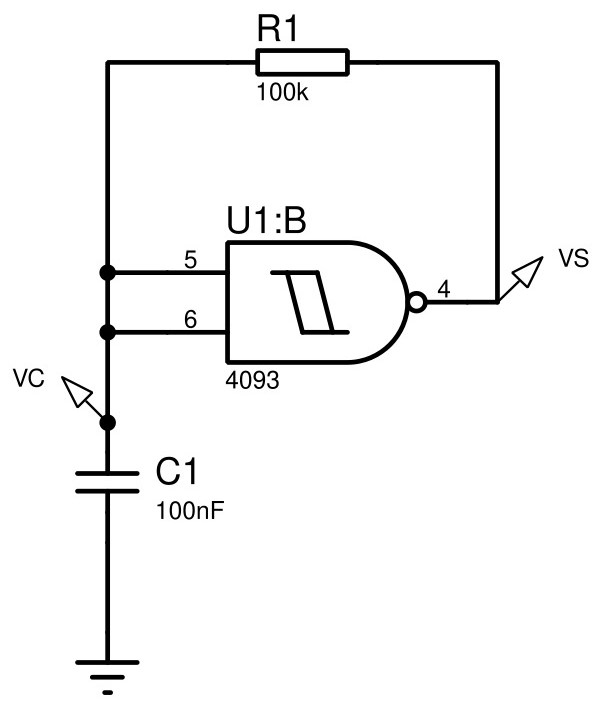
\includegraphics{./Circuits/C1.jpeg}
                
                \caption{Astable NAND Logic Gate Circuit}
                
            }
        }
        
        \ffigbox{
            \adjustbox{scale=0.8}{
                \begin{tikzpicture}
                    \begin{axis}[
                            legend pos=south east,
                            legend entries={$V_s$, $V_c$},
                            axis lines = middle,
                            ytick={15,12.5, 10, 7.5, 5, 2.5, 0, -2.5, -5, -7.5, -10, -12.5, -15},
                            yticklabels={ , ,10, , 5, , 0, , -5, , -10, , },
                            xtick={-0.015, -0.0125, -0.01, -0.0075, -0.005, -0.0025, 0.0025, 0.005, 0.0075, 0.01, 0.0125, 0.015},
                            xticklabels={ -15 , , -10, , -5, , , 5, , 10, ,15 },
                            xmin=-0.012, xmax=0.012,
                            ymin=-3, ymax=16, height=0.3\textwidth, width=0.5\textwidth,
                            change x base,
                            x SI prefix=milli,x unit=s,
                            ylabel=\large{$V$},
                            label style ={at={(ticklabel cs:1.15)}}]
                        
                        \addplot[orange, smooth] table[x=TIME, y=Vs, col sep=space]{./Data/1.txt};
                        \addplot[blue, smooth] table[x=TIME, y=Ve, col sep=space]{./Data/1.txt};
                    \end{axis}
                \end{tikzpicture}
                \caption{Signal Response $V_c$ and $V_s$}
            }
        }
        
    \end{floatrow}
\end{figure}

According to theory, while the logic gate outputs $+15V$, pin 5 will be set to \verb|HIGH|, and the capacitor will start charging itself. When the capacitor meets its threshold voltage $9.4V$ the output flops to $0V$ at which point pin 5 is set to \verb|LOW| and pin 6 discharges from \verb|HIGH| until the negative threshold volatge of $7.3V$.

This cycle repeats itself indefinetely creating a clock which can be seen on the signal response graph, and corresponds to the theoretical values.

\subsection{Astable with NAND Logic Gate (4011)}

\begin{figure}[ht]
    \begin{floatrow}
        \ffigbox{
            \adjustbox{scale=0.8}{
            
                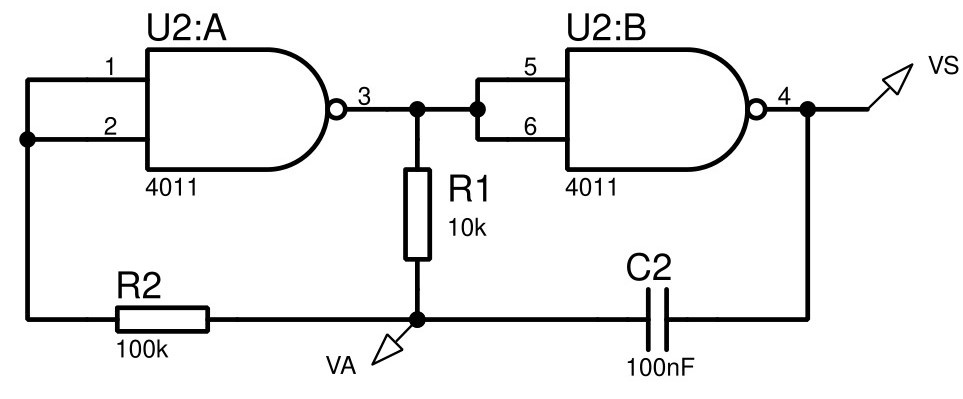
\includegraphics{./Circuits/C2.jpeg}
                
                \caption{Astable NAND Logic Gate Circuit}
                
            }
        }
        
        \ffigbox{
            \adjustbox{scale=0.8}{
                \begin{tikzpicture}
                    \begin{axis}[
                            legend pos=south east,
                            legend entries={$V_a$, $V_s$,$V_c$,$V_b$},
                            axis lines = middle,
                            ytick={17.5, 15, 12.5, 10, 7.5, 5, 2.5, 0, -2.5, -5, -7.5, -12.5, -15},
                            yticklabels={ , 15, ,10, , 5, , 0, , -5, , , , },
                            xtick={-0.004, -0.003, -0.002, -0.001, 0.001, 0.002, 0.003, 0.004, 0.005},
                            xticklabels={ -4, , -2, , , , 2, , 4, ,},
                            xmin=-0.0032, xmax=0.0038,
                            ymin=-10, ymax=20, height=0.3\textwidth, width=0.5\textwidth,
                            change x base,
                            x SI prefix=milli,x unit=s,
                            ylabel=\large{$V$},
                            label style ={at={(ticklabel cs:1.15)}}]
                        
                        \addplot[blue, smooth] table[x=TIME, y=Vs, col sep=space]{./Data/2.txt};
                        \addplot[orange, smooth] table[x=TIME, y=Ve, col sep=space]{./Data/2.txt};
                        \addplot[red, smooth] table[x=TIME, y=Vc, col sep=space]{./Data/2.txt};
                        \addplot[green, smooth] table[x=TIME, y=Va, col sep=space]{./Data/21.txt};
                    \end{axis}
                \end{tikzpicture}
                \caption{Signal Response $V_a$, $V_b$, $V_c$ and $V_s$}
            }
        }
        
    \end{floatrow}
\end{figure}

Inicially the logic gates output $15V$ on pin 4 and pin 3. This in turn charges the capacitor allowing current to pass through and results in a spike in voltage at $V_a$, setting logic levels at pin 1 and 2 to \verb|HIGH|, returning $0V$  at output 3.

As the voltage spike $V_a$ falls down to the threshold $6.8V$ for pins 5 and 6 the logic gate outputs $0V$ on pin 4, discharging the capcitor. A negative voltage spike on $V_a$ is then induced due to the capacitor, the output on pin 3 then flips to  $15V$ setting pin 6 to a \verb|LOW| logic level until the voltage rises to the $6.8V$ threshold as a result of the discharging capacitor.

This cycle repeats itself indefinetely creating a clock which can be seen on the signal response graph, and corresponds to the theoretical values.

\begin{figure}[ht]
    \begin{floatrow}
        \ffigbox{
            \adjustbox{scale=0.8}{
            
                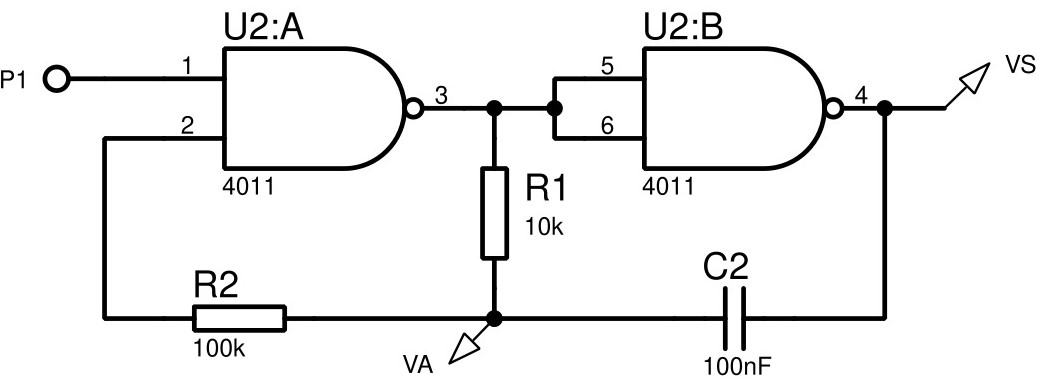
\includegraphics{./Circuits/C21.jpeg}
                
                \caption{Astable NAND Logic Gate Circuit with Enable Probe}
                
            }
        }
        
        \ffigbox{
            \adjustbox{scale=0.8}{
                \begin{tikzpicture}
                    \begin{axis}[
                            legend pos=south east,
                            legend entries={$V_s$ (H), $V_a$ (H),$V_s$ (L),$V_a$ (L)},
                            axis lines = middle,
                            ytick={17.5, 15, 12.5, 10, 7.5, 5, 2.5, 0, -2.5, -5, -7.5, -12.5, -15},
                            yticklabels={ , 15, ,10, , 5, , 0, , -5, , , , },
                            xtick={-0.004, -0.003, -0.002, -0.001, 0.001, 0.002, 0.003, 0.004, 0.005},
                            xticklabels={ -4, , -2, , , , 2, , 4, ,},
                            xmin=-0.0032, xmax=0.0038,
                            ymin=-10, ymax=20, height=0.3\textwidth, width=0.5\textwidth,
                            change x base,
                            x SI prefix=milli,x unit=s,
                            ylabel=\large{$V$},
                            label style ={at={(ticklabel cs:1.15)}}]
                        
                        
                        \addplot[orange, smooth] table[x=TIME, y=Vs, col sep=space]{./Data/22H.txt};
                        \addplot[blue, smooth] table[x=TIME, y=Va, col sep=space]{./Data/22H.txt};
                        \addplot[gray, smooth] table[x=TIME, y=Vs, col sep=space]{./Data/22L.txt};
                        \addplot[green, smooth] table[x=TIME, y=Va, col sep=space]{./Data/22L.txt};
                        
                    \end{axis}
                \end{tikzpicture}
                \caption{Signal Response $V_a$ and $V_s$ for P1 High and Low}
            }
        }
        
    \end{floatrow}
\end{figure}

As the probe \verb|P1| is set to a \verb|HIGH| logic state, the circuit appears to be functionning properly with no issues. The same however is not to be said when \verb|P1| is at a \verb|LOW| logic state, in which case the astable circuit no longer outputs a clock signal.

Due to this particular functionality we can quickly spot that \verb|P1| acts as an enabling signal that can decide whether to turn the clock on or off. 

\subsection{Astable with NE555}


\begin{figure}[ht]
    \begin{floatrow}
        \ffigbox{
            \adjustbox{scale=0.8}{
            
                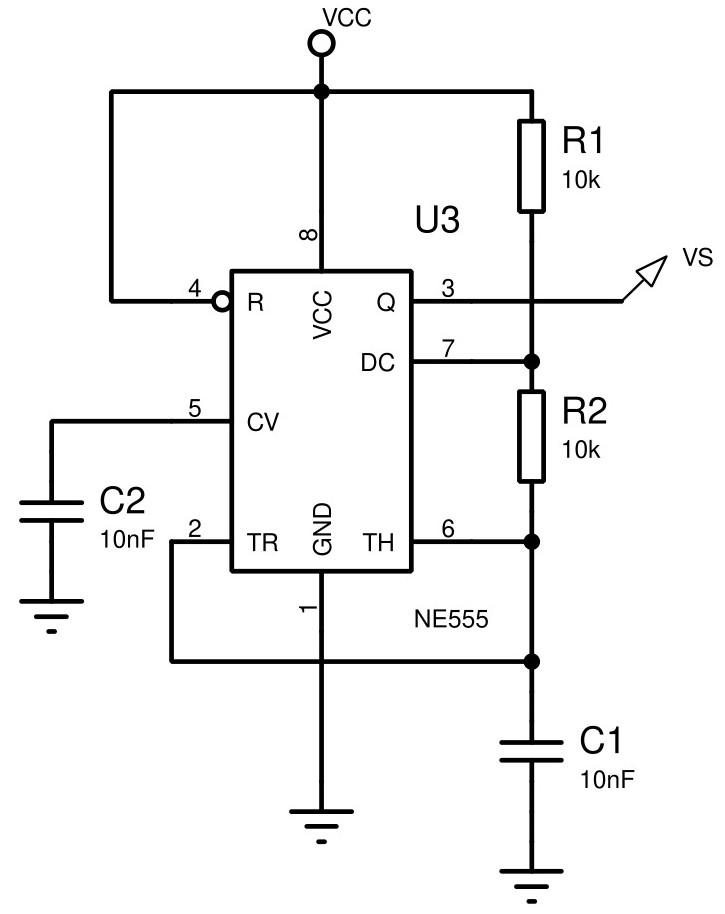
\includegraphics{./Circuits/C3.jpeg}
                
                \caption{Astable NE555 Circuit}
                
            }
        }
        
        \ffigbox{
            \adjustbox{scale=0.8}{
                \begin{tikzpicture}
                    \begin{axis}[
                            legend pos=south east,
                            legend entries={$V_s$, $V_c$},
                            axis lines = middle,
                            ytick={17.5, 15, 12.5, 10, 7.5, 5, 2.5, 0, -2.5, -5, -7.5, -12.5, -15},
                            yticklabels={ , 15, ,10, , 5, , 0, , -5, , , , },
                            xtick={0.0006, 0.00065, 0.0007, 0.00075, 0.0008, 0.00085, 0.0009, 0.00095, 0.001},
                            xticklabels={ 600, , 700, , 800, , 900, , ,},
                            xmin=0.00055, xmax=0.001,
                            ymin=-10, ymax=20, height=0.3\textwidth, width=0.5\textwidth,
                            change x base,
                            x SI prefix=micro,x unit=s,
                            ylabel=\large{$V$},
                            label style ={at={(ticklabel cs:1.15)}}]
                        
                        
                        \addplot[orange, smooth] table[x=TIME, y=Vs, col sep=space]{./Data/3.txt};
                        \addplot[blue, smooth] table[x=TIME, y=Va, col sep=space]{./Data/3.txt};
                        
                        \draw[orange,dashed] (0.000584,-10) -- (0.000584,20);
                        \draw[orange,dashed] (0.000655,-10) -- (0.000655,20);
                        \draw[orange, dashed] (0.000802,-10) -- (0.000802,20);
                        
                        \draw[orange, stealth-stealth] (0.000594, 16) -- (0.000645, 16);
                        \draw[orange, stealth-stealth] (0.000665, 16) -- (0.000792, 16);
                        
                        
                        \node at (0.000619,18) {\large{$T_L$}};
                        \node at (0.000728,18) {\large{$T_H$}};                   
                    \end{axis}
                    
                \end{tikzpicture}
                \caption{Signal Response $V_c$ and $V_s$}
            }
        }
        
    \end{floatrow}
\end{figure}

After having set the circuit up, we carefully measure $T_L=70\ \mu s$ and $T_H=148\ \mu s$ with which we deduce the period $T=T_H+T_L=218\ \mu s$ and by extension the frequency $f=\frac{1}{T}=4.6\ kH_z$. The duty cycle can be easily obtained as $\tau=\frac{T_H}{T}=67.9\%$\\
Level triggers are also measured to be around $10.2V$ for the positive threshold and $4.8V$ for the negative threshold.

\begin{figure}[ht]
    \begin{floatrow}
        \ffigbox{
            \begin{tabular}{|c|c|}
                \hline
                Properties       & Values       \\
                \hline
                $T_H$            & $148\ \mu s$ \\
                $T_L$            & $70\ \mu s$  \\
                \hline
                Period           & $218\ \mu s$ \\
                \hline
                Duty Cycle       & $67.9\ \%$   \\
                \hline
                Frequency        & $4.6\ kH_z$  \\
                \hline
                Positive Trigger & $10.2\ V$    \\
                Negative Trigger & $4.8\ V$     \\
                \hline
                
            \end{tabular}
            \caption{Measured Properties Summary}
        }
        
        \ffigbox{
            \begin{tabular}{|c|c|}
                \hline
                Properties       & Values        \\
                \hline
                $T_H$            & $138\ \mu s$  \\
                $T_L$            & $69.3\ \mu s$ \\
                \hline
                Period           & $231\ \mu s$  \\
                \hline
                Duty Cycle       & $66.5\ \%$    \\
                \hline
                Frequency        & $4.5\ kH_z$   \\
                \hline
                Positive Trigger & $10\ V$       \\
                Negative Trigger & $5\ V$        \\
                \hline
                
            \end{tabular}
            \caption{Datasheet Properties Summary}
        }
        
    \end{floatrow}
\end{figure}

All mesured values correspond with those from the datasheet.

As the \verb|Trigger| voltage rises due to the charging capacitor, the comparator compares its value to the threshold $\frac{2}{3}V_{CC}$, as it does the voltage outputed to the flipflop sets the \verb|Output| to \verb|+VCC|. 

Once it reaches the threshold the capacitor starts to discharge and the comparator no longer outputs to the flipflop causing the second comparator to compare its value to the \verb|Threshold|, and since the latter is alway above $\frac{1}{3}V_{CC}$ the \verb|Output| signal is set to $0V$. Upon meeting the $\frac{1}{3}V_{CC}$ threshold the cycle then repeats itself as the capcitor charges and \verb|Output| is set back to \verb|+VCC|.

This process can be seen on the signal response graph, as the capacitor charges, $V_s$ is at $15V$, and as it discharges, i$V_s$ falls down to $0V$.

This type of astable circuit is particularly useful since the pulse width can easily be modulated by changing the values of the resistors or capacitors using the datasheet as a refferal.

\subsection{Astable with Operational Amplifier}

\begin{figure}[ht]
    \begin{floatrow}
        \ffigbox{
            \adjustbox{scale=0.8}{
            
                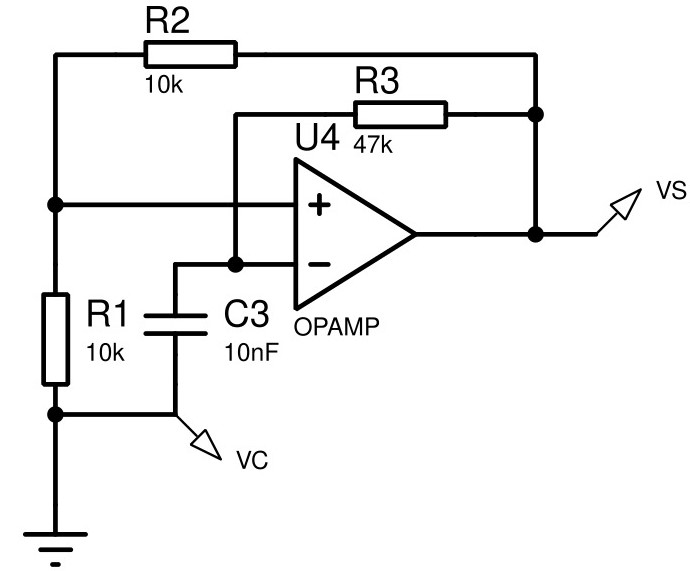
\includegraphics{./Circuits/C4.jpeg}
                
                \caption{Astable Operational Amplifier Circuit}
                
            }
        }
        
        \ffigbox{
            \adjustbox{scale=0.8}{
                \begin{tikzpicture}
                    \begin{axis}[
                            legend pos=south east,
                            legend entries={$V_s$, $V_c$},
                            axis lines = middle,
                            ytick={ 15, 12.5, 10, 7.5, 5, 2.5, 0, -2.5, -5, -7.5, -10, -12.5, -15},
                            yticklabels={ 15, ,10, , 5, , , , -5, , -10, , -15},
                            xtick={-0.0004, -0.0002, 0.0002, 0.0004, 0.0006, 0.0008, 0.001, 0.0012, 0.0014, 0.0016, 0.0018},
                            xticklabels={ -4, , , 4, , 8, , 12, , 16, , },
                            xmin=-0.00045, xmax=0.002,
                            ymin=-16, ymax=16, height=0.3\textwidth, width=0.5\textwidth,
                            change x base,
                            x SI prefix=micro,x unit=s,
                            ylabel=\large{$V$},
                            label style ={at={(ticklabel cs:1.15)}}]
                        
                        
                        \addplot[orange, smooth] table[x=TIME, y=Vs, col sep=space]{./Data/4.txt};
                        \addplot[blue, smooth] table[x=TIME, y=Vc, col sep=space]{./Data/4.txt};
                        
                    \end{axis}
                    
                \end{tikzpicture}
                \caption{Signal Response $V_c$ and $V_s$}
            }
        }
        
    \end{floatrow}
\end{figure}

As the operational amplifier incicially outputs $15V$, a positive threshold value $7.5V$ is set on the positive input pin whilst on the negative pin the capacitor charges itself from $0V$. Upon reaching the set threshold, the output flops to $-15V$ setting the negative threshold value at $-7.5V$. 

As a result of the negative voltage the capacitor discharges itself until  the negative threshold to which point the cycle repeats itself as the output of the operational amplifier is back at $15V$.

This process can be seen on the signal response graph, as the capacitor charges, $V_s$ is at $15V$, and as it discharges, $V_s$ falls down to $-15V$.


\section{Summary}

\begin{enumerate}
    \item The first circuit with the NAND logic gate (4093) is convenient as it requires minimal component to set a function clock, with so however, the pulse width modulation needs to be repeatedly calculated and the circuit itself offers no signal input that can act as an enbaling function for the clock.
    \item The second circuit with the NAND logic gate (4011) offer the same features as the previous 4093 NAND gate, in addition to the possibility to enable to clock using an external signal input at \verb|P1|. The main drawback being that it requires two logic gates which can result in being more costly for extensive fabrication.
    \item The NE555 Circuit is much more expensive in terms of cost as the component alone uses 1 flipflop, 2 comparators, and 2 transistor. This comes with a glad payoff were the clock itself can be easily mended with as the pulse width modulation is documented as well as its frequency and trigger levels. The component itself is very versatile and offers many more adjustable functions that other circuits do not have.
    \item   Lastly, the astable operational amplifier circuit allows for a similar clock as the NAND logic gate (4093), although benefiting from high slew rate and wide output voltage range. With its counterpart it still lacks an enabling input and requires manual computation for its pulse width modulation.
\end{enumerate}










\end{document}